\documentclass{standalone}
\usepackage{pgfplots}
\pgfplotsset{compat=newest}
\begin{document}
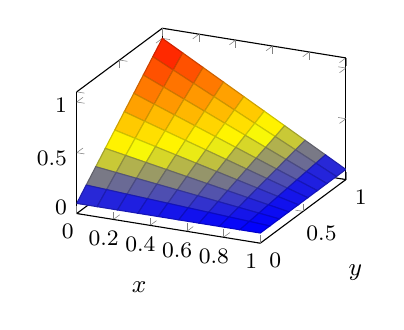
\begin{tikzpicture}
	\begin{axis}[footnotesize,xlabel=$x$,ylabel=$y$,unit vector ratio=]
	\addplot3[surf,samples=10,domain=0:1] {(1-x)*y};
	\end{axis}
\end{tikzpicture}
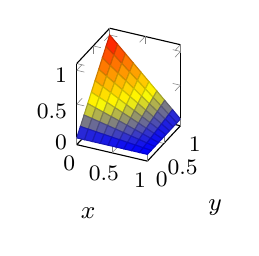
\begin{tikzpicture}
	\begin{axis}[footnotesize,xlabel=$x$,ylabel=$y$,
		unit rescale keep size=false,
		unit vector ratio=1 1 1]
	\addplot3[surf,samples=10,domain=0:1] {(1-x)*y};
	\end{axis}
\end{tikzpicture}
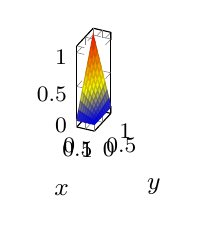
\begin{tikzpicture}
	\begin{axis}[footnotesize,xlabel=$x$,ylabel=$y$,
		unit vector ratio*=0.25 0.5, % the '*' implies 'unit rescale keep size=false'
	]
	\addplot3[surf,samples=10,domain=0:1] {(1-x)*y};
	\end{axis}
\end{tikzpicture}
\end{document}
